\chapter[Fundamentação Teórica]{Fundamentação Teórica}

\section{Imagens Digitais}

Segundo \cite{young1998fundamentals}, uma imagem pode ser representada como uma função de duas variáveis reais, por exemplo, \textit{a(x,y)} com \textit{a} sendo a amplitude (ex.: brilho) da imagem nas coordenadas reais de posição \textit{(x,y)}. As amplitudes da imagem serão sempre dadas por um conjunto de números reais ou inteiros, sendo este último o resultado de um processo de quantização, que converte uma faixa de números reais, por exemplo de 0,0 a 100,0\%, em um número discreto de níveis.

De acordo com o mesmo autor, imagens digitais a(m,n), descritas em um espaço discreto, são obtidas a partir de imagens analógicas a(x,y), por sua vez descritas em um espaço contínuo,  através do processo de amostragem. A equação \ref{eq1} ilustra uma possível representação matricial para uma imagem digital.
\vspace{-1cm}
\begin{center}
	\begin{equation}
	a =
	\begin{bmatrix}
  		a_{0,0} & a_{0,1} & \cdots & a_{0,n-1} \\
  		a_{1,0} & a_{1,1} & \cdots & a_{1,n-1} \\
  		\vdots  & \vdots  & \ddots & \vdots  \\
  		a_{m,0} & a_{m,1} & \cdots & a_{m-1,n-1}
	\end{bmatrix}.
	\label{eq1} 
	\end{equation}
\end{center}


\subsection{Imagens Monocromáticas}
	
	De acordo com \cite{gonzalez2004digital}, o processo de digitalização das imagens requer uma amostragem espacial, este processo irá definir as quantidades $M$ de linhas e $N$ de colunas que caracterizam o espaço discreto em que a imagem está contida, além do número $L$, que no caso das imagens monocromáticas é o número de tons de cinza que cada \textit{pixel} (elemento da imagem) pode assumir. $M$ e $N$ devem ser números inteiros e positivos. Entretanto, devido ao processamento, armazenamento e considerações do hardware de amostragem, o número de níveis de cinza é tipicamente uma potência inteira de 2:
\vspace{-1cm}
\begin{center}
	\begin{equation}
		L = 2^K,
	\end{equation}
\end{center}	 
\noindent onde $K$ é um valor inteiro positivo. Assumindo que os níveis de cinza são representados por números inteiros igualmente espaçados no intervalo [0,L-1], o número de \textit{bits} $B$ necessários para armazenar uma imagem digitalizada é:

\begin{equation}
	b = M \times N \times K.
\end{equation}

\subsection{Representação de Cenas Naturais e Sintéticas}

Uma cena de vídeo natural é geralmente composta de vários objetos, cada um com suas características próprias (forma, profundidade, textura e iluminação). A cor e o brilho de uma cena de vídeo natural mudam com diferentes graus de intensidade em toda a cena, ou seja, tem tons contínuos. Uma cena sintética, por sua vez, procura emular uma cena real ou apresentar uma cena virtual, e é geralmente desenvolvida com métodos de computação gráfica \cite{scharstein2002taxonomy}. 

\begin{figure}[h]
    \centering
    \subfloat[]{
	    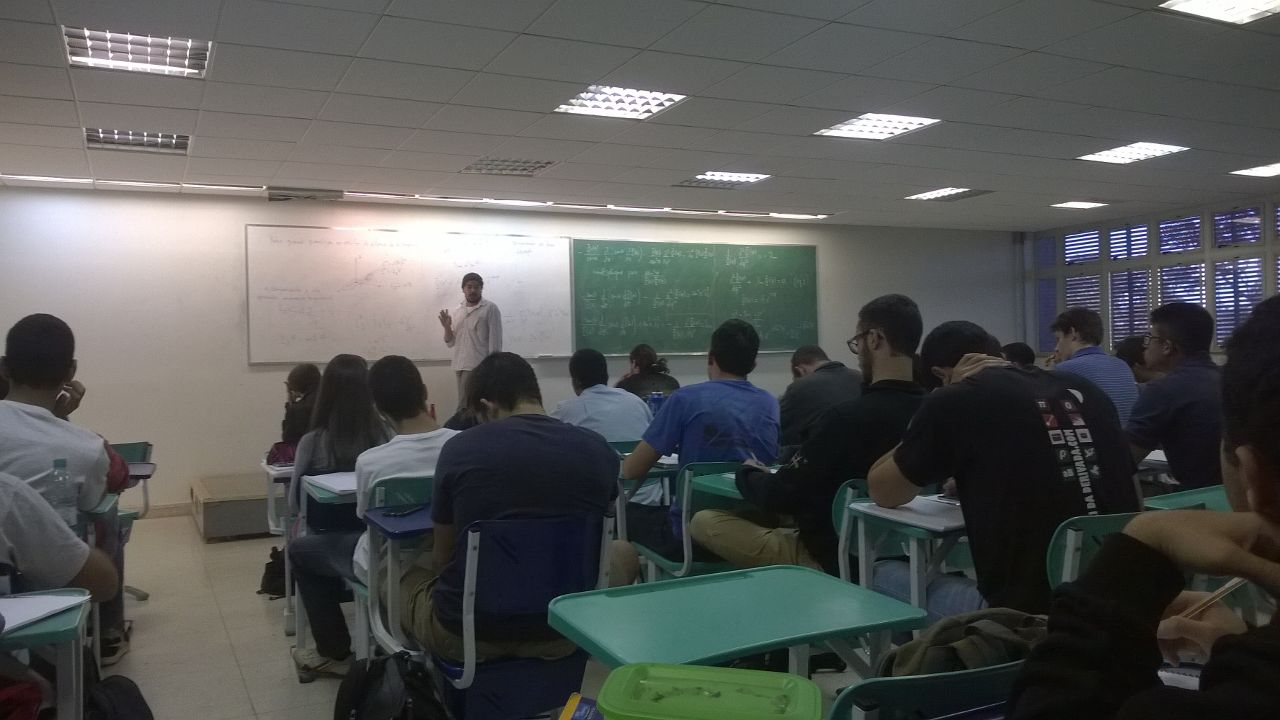
\includegraphics[width=0.4\linewidth]{figuras/CENA_NATURAL.jpg}\label{fig:original}
    }
    \qquad
    \subfloat[]{
    	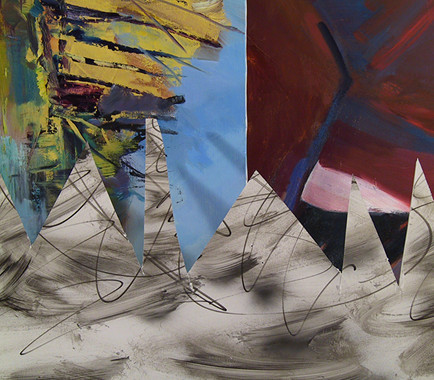
\includegraphics[width=0.4\linewidth]{figuras/CENA_SINTETICA.jpg}\label{fig:red}
    }
    \caption{Cenas: (a) natural; (b) sintética.}%
	    
    \label{fig:RGB}%
\end{figure}

Segundo \cite{garcia2013tecnicas}, para se representar cenas naturais e sintéticas de forma digital é necessário amostrá-las no espaço e no tempo, como mostrado na Figura \ref{AMOSTRAGEM_VIDEO}. Para isso, são obtidas fotografias digitais das cenas (quadros) entre intervalos regulares.

\begin{figure}[h]
	\centering
	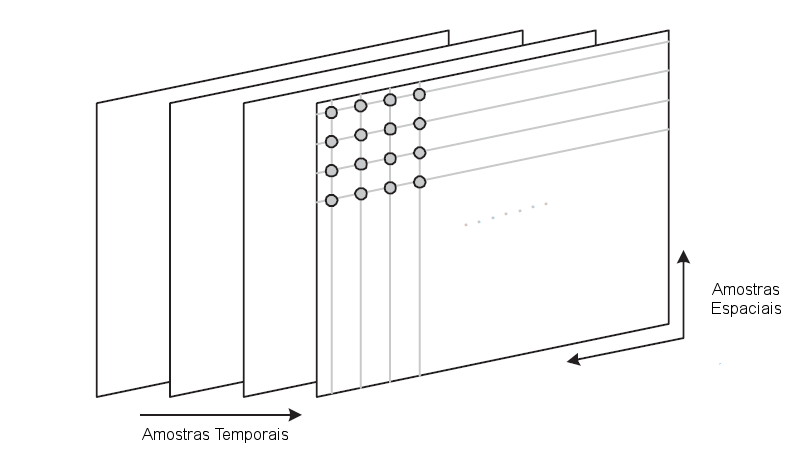
\includegraphics[scale=0.65]{figuras/AMOSTRAGEM_VIDEO.png}
	\caption{Amostragem espacial e temporal de uma sequência de vídeo.}
	\label{AMOSTRAGEM_VIDEO}
\end{figure}

\subsection{Conceito de Resolução} \label{resolucao}


Ainda de acordo com \cite{gonzalez2004digital}, temos que definir o conceito de resolução espacial e de tons de cinza. Sabe-se que a resolução espacial está relacionada ao menor detalhe discernível em uma imagem. Suponha que deseja-se construir um gráfico com linhas verticais de largura W, e que o espaço entre essas linhas possuam a mesma largura W. Um par de linhas é constituído por uma linha vertical e seu respectivo espaço adjacente. Portanto, a largura de um par de linhas é 2W e existem 1/2W pares de linha por unidade de distância. Ou seja, a resolução espacial representa o nível de detalhe que uma imagem comporta, ou ainda quantifica quão próximas as linhas podem ficar umas das outras, sendo que o principal fator determinante da resolução espacial de uma imagem é o processo de amostragem. Já a resolução de tons de cinza \textit{hardware}, assim como a espacial, é definida como a menor mudança discernível entre os tons de cinza. No entanto medir essas mudanças é um processo com um nível de subjetividade maior. Devido a considerações sobre o \textit{hardware}, tem-se que o número de níveis de cinza é uma potência de 2, como já foi dito. Na maioria dos casos utilizam-se 8 \textit{bits} ou 16 \textit{bits} (em aplicações em que é necessária uma gama maior de níveis). Em certos casos pode-se deparar com imagens digitalizadas com 10 ou 12 \textit{bits} de precisão, mas estes casos são exceções a regra geral.


\subsection{Espaço de Cores}

De acordo com \cite{richardson2011h}, na maioria das aplicações com vídeos e imagens digitais é necessário trabalhar e exibir imagens coloridas, o que faz necessário um mecanismo para capturar e representar a informação das cores. Uma imagem monocromática requer apenas um número que indique o brilho ou a luminância de cada amostra espacial. Imagens coloridas, por outro lado, requerem no mínimo três números por pixel para representar com precisão a cor. O método escolhido para representar o brilho, luminância e cores é chamado espaço de cores.

\subsubsection{O sistema de cores RGB}

No espaço de cores RGB, a cor das amostras da imagem é representadas por três números que significam proporções relativas de vermelho (\textit{\textbf{R}ed}), verde (\textit{\textbf{G}reen}) e azul (\textit{\textbf{B}lue}), essas são as três cores primárias aditivas da luz \cite{richardson2011h}.	Combinando vermelho, verde e azul em variadas proporções pode-se criar qualquer cor. A figura \ref{fig:RGB} é um exemplo de representação dos componentes vermelho, verde e azul de uma imagem colorida. A componente vermelha(figura \ref{fig:RGB} - b) consistem em todas as amostras vermelhas da imagem, a componente verde (figura \ref{fig:RGB} - c) consistem em todas as componentes verdes das imagem e por fim a componente azul contendo todos os amostras azuis da imagem (figura \ref{fig:RGB} - d).

\begin{figure}
    \centering
    \subfloat[]{
	    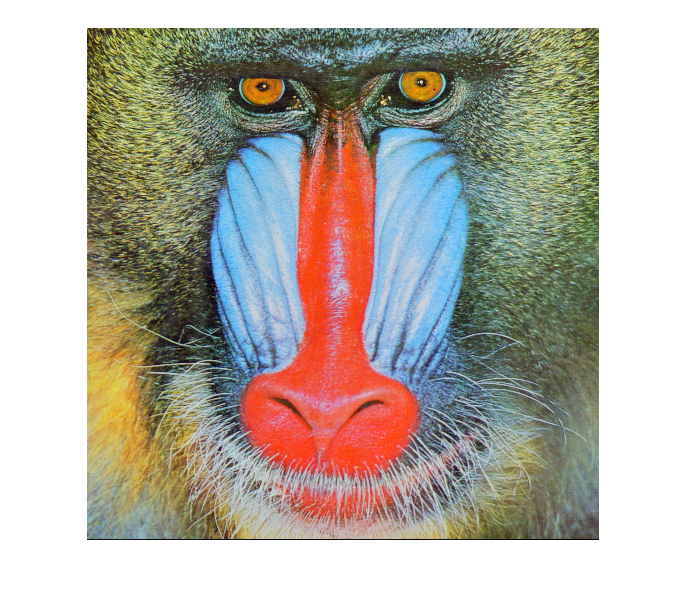
\includegraphics[width=0.4\linewidth]{figuras/MANDRIL.png}\label{fig:original}
    }
    \qquad
    \subfloat[]{
    	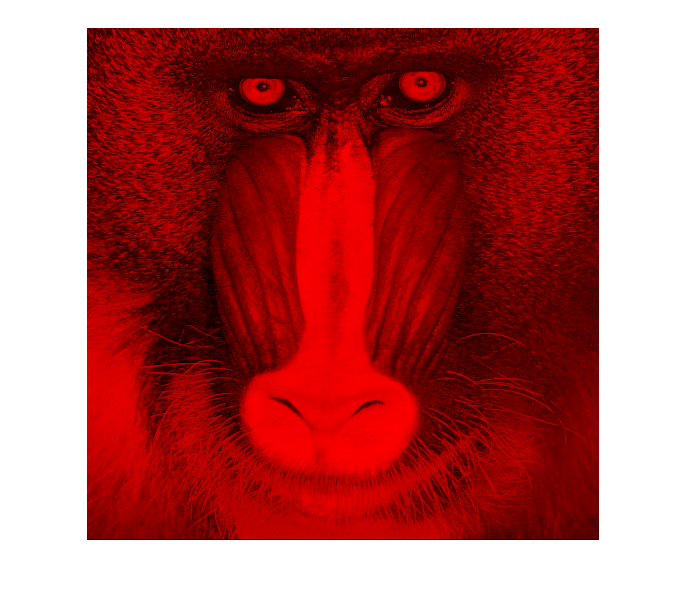
\includegraphics[width=0.4\linewidth]{figuras/COMPONENTE_VERMELHA.png}\label{fig:red}
    }
	\qquad
    \subfloat[]{
    	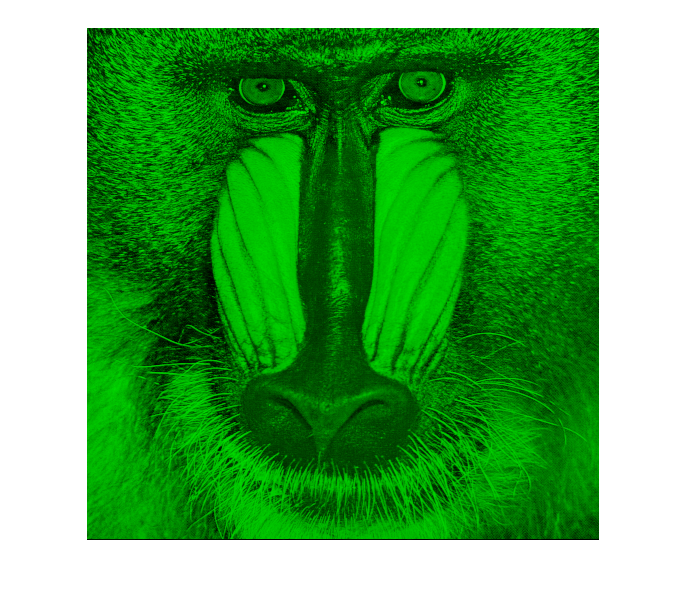
\includegraphics[width=0.4\linewidth]{figuras/COMPONENTE_VERDE.png}\label{fig:green}
    }
	\qquad
    \subfloat[]{
    	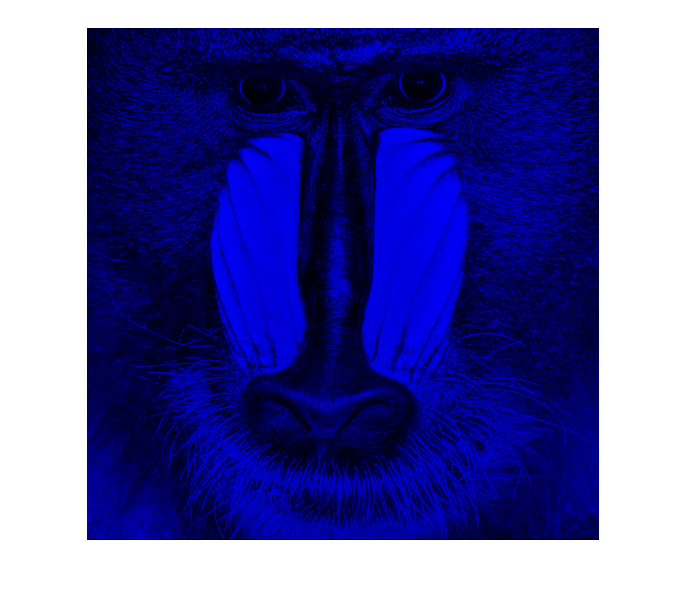
\includegraphics[width=0.4\linewidth]{figuras/COMPONENTE_AZUL.png}\label{fig:blue}
    }
    \caption{Componentes no espaço RBG: (a) imagem original; (b) vermelho; (c) verde; (d) azul.}%
	    
    \label{fig:RGB}%
\end{figure}

Para o mesmo autor, o espaço de cor RGB é bem adequado para capturar e exibir imagens coloridas. Obter uma imagem RGB envolve filtrar os componentes vermelho, verde e azul da cena e capturar cada um com um conjunto de sensores separado. Para exibir as cores de uma imagem RGB ilumina-se separadamente as componentes vermelha, verde e azul de cada pixel de acordo com a intensidade de cada componente. A partir de uma certa distância de visualização, os componentes separados se fundem para dar a aparência da cor \enquote{verdadeira}. 

\subsubsection{O sistema de cores YCrCb}
O sistema visual humano é menos sensível a cor do que à luminância. No espaço RGB as três cores são igualmente importantes e, assim, são normalmente armazenadas todas com a mesma resolução, mas é possível representar uma imagem colorida mais eficientemente através da separação da luminância a partir da informação da cor \cite{richardson2011h}.

O YCrCb é um espaço de cor definido pela CCIR (\textit{International Consultative Committee on Broadcasting}), também referido como o espaço de cor CCIR 601 \cite{acharya2002integrated}. YCrCb define a informação  das imagens coloridas  em termos da luminância (componente Y) e de dois valores de crominância diferentes (Cr-crominância de cores vermelhas e Cb-crominância de cores azul) e não como uma combinação de cores como no espaço RGB. Quando cada pixel é representado assim, ao contrário do espaço de cor RGB em que cada pixel tem, tipicamente, 24 \textit{bits} de informação (8 \textit{bits} para cada plano de cor), cada pixel pode ser representado por apenas 12 \textit{bits} devido a redundância da informação de crominância. Para isso, primeiro deve-se converter do espaço RGB (24 \textit{bits}/\textit{pixel}) para YCrCb (24 \textit{bits}/\textit{pixel}), da seguinte maneira:

\begin{center}
	\begin{equation}
	\begin{split}
	\begin{bmatrix}		
	Y\\ Cr \\ Cb
	\end{bmatrix}
	 = 
	\begin{bmatrix}
  		0,299 & 0,587 &  0,114 \\
  		-0,169 &-0.331 & 0,5 \\
  		0,5  & -0.419  & -0.091\\
	\end{bmatrix}
	\begin{bmatrix}
	R\\ G \\ B
	\end{bmatrix}
	\label{rgb2yuv} 
	\end{split}
	\end{equation}

\end{center}

\noindent Após o processo de conversão, pode-se dizimar os \textit{pixels} de Cr e Cb de modo que só um a cada quatro \textit{pixels} permaneça representando os quatro. Ainda é possível subamostrar Cr e Cb com fator de 2, tanto na horizontal como na vertical.


\section{Mudança de resolução de imagens}



A mudança arbitrária de resolução de imagens, surge com bastante frequência em diversas aplicações. Por exemplo, imagens e vídeos muitas vezes precisam ser redimensionados espacialmente, a fim de garantir que os dados possam trafegar nas redes de comunicações sobre as quais eles viajam e serem exibidos nos dispositivos de exibição do usuário final sobre o qual eles vão ser apresentados \cite{salazar2007complexity}.

O aumento ou redução da resolução de imagens são obtidas através de processos de decimação ou interpolação \cite{diniz2010digital}. 

\subsection{Decimação}

O processo de decimação de uma imagem por um fator $M$ consiste em manter uma linha a cada $M$ linhas e o mesmo para as colunas. Definindo $u$ e $v$ como sendo as coordenadas de largura e comprimento de uma dada imagem, cada \textit{pixel} da imagem original é indicada por $I(u,v)$ , e cada \textit{pixel} da imagem decimada por $M$ é indicado por $I^D(u,v)$  (garcia2013tecnicas). Assim, temos:

\begin{equation}
I^D(u,v) = I(uM,uV) 
\label{eq_decimacao}
\end{equation}

Aplicando a transformada de Fourier sobre a equação \ref{eq_decimacao} prova-se que $I^D(u,v)$ sofrerá superposição espectral ( ou \textit{aliasing}, em inglês), se a largura da faixa da transformada discreta de Fourier  de $I(u,v)$ estiver fora do intervalo $\left[-\frac{\pi}{M},\frac{\pi}{M} \right]$. Para evitar que isso aconteça, o processo de decimação é geralmente precedido por uma filtragem que preserve o intervalo, como mostrado no diagrama de blocos da Figura \ref{fig:deci2} \cite{garcia2013tecnicas} . \\

\begin{figure}[h]
    \centering
    \subfloat[]{
	    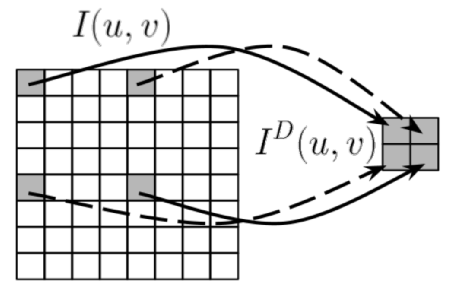
\includegraphics[width=0.4\linewidth]{figuras/decimacao_1.png}\label{fig:deci1}
    }
    \qquad
    \subfloat[]{
    	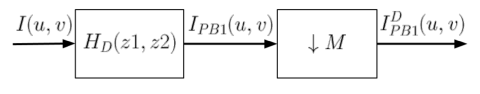
\includegraphics[width=0.4\linewidth]{figuras/decimacao_2.png}\label{fig:deci2}
    }
    \caption{(a) decimação $I_D(u,v)$ de uma imagem $I^D(u,v)$ de tamanho 8x8 por um fator 4; (b) operação geral de decimação: a imagem $I(u,v)$ é convoluída com o filtro $H_D(z1,z2)$, gerando uma versão passabaixas $I^D_{PB1}$, e depois decimada por um fator M, gerando uma versão $I(u,v)$ de menor resolução \cite{garcia2013tecnicas}. }%
	    
\end{figure}

\subsection{Interpolação}

    O processo de interpolação de uma imagem por um fator $M$ consiste em acrescentar $M-1$ zeros entre cada linha e $M-1$ também zeros entre cada coluna da imagem, como mostrado na Figura \ref{fig:inter1}. Definindo a imagem interpolada por $M$ como sendo $I^I(u,v)$, então temos:

\begin{equation}
\begin{matrix}
	I^I(u,v)=\Bigg\{
	\begin{matrix}
		I(u/M,v/M), & u = jM \quad e \quad v = kM, \quad j,k \in  \mathbb{Z}\\ 
		0, &  \textrm{caso contrário}
	\end{matrix}
\end{matrix}
\label{eq_inter}
\end{equation}


Aplicando a transformada de Fourier sobre a equação \ref{eq_inter}, prova-se que $I^I(u,v)$ deverá ser posteriormente filtrada por um filtro passabaixas para evitar problemas de superposição espectral. O filtro, denominado $H_I(u,v)$, deverá ter ganho igual a $M$ no intervalo de frequências $\left[-\frac{\pi}{M},\frac{\pi}{M} \right]$, e ganho nulo em todas as outras frequências. A Figura \ref{fig:inter2} ilustra a operação geral de interpolação por um fator $M$, incluindo o filtro passabaixas $H_I$ \cite{garcia2013tecnicas}. 


\begin{figure}[h]
    \centering
    \subfloat[]{
	    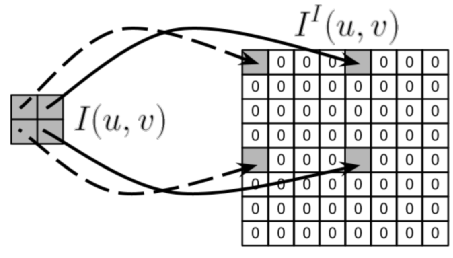
\includegraphics[width=0.4\linewidth]{figuras/interpolacao_1.png}\label{fig:inter1}
    }
    \qquad
    \subfloat[]{
    	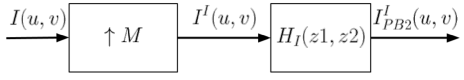
\includegraphics[width=0.4\linewidth]{figuras/interpolacao_2.png}\label{fig:inter2}
    }
    \caption{(a) interpolação $I^I(u,v)$ de uma imagem $I(u,v)$ de tamanho 2x2 por um fator 4; (b) operação geral de interpolação: a imagem $I(u,v)$ é interpolada por um fator $M$ e depois convoluída com o $H_I$, gerando uma versão em maior resolução de $I(u,v)$ \cite{garcia2013tecnicas}. }%
	    
\end{figure}

\subsection{Transformadas Discretas de Cosseno}
 \label{DCT}
Desde que muito material multimídia passou a ser comprimido usando as populares transformadas discretas de cosseno (DCT, do inglês \textit({Discrete cosine transform}), como nos padrões JPEG, MPEG e H.26X, uma operação de redimensionamento espacial que seja eficiente, flexível computacionalmente e que possa ser realizado no domínio da DCT é desejável. Flexibilidade computacional é especialmente importante porque uma ampla gama de opções de projeto muitas vezes se faz necessária, a fim de atender requisitos como consumo energético e performace.
\cite{salazar2007complexity}
Segundo \cite{T.81}, a transformada discreta de cosseno (DCT), é uma transformada matemática que tem como funções de base os cossenos, por meio dela converte-se um bloco de amostras em um bloco correspondente de coeficientes da transformada. Essa operação é dividida em duas operações, a transformada direta (ou FDCT, do inglês \textit{Forward discrete cosine transform}), mostrada abaixo:

\vspace{-3mm}
\begin{equation}
	\label{FDCT}
	Y = AXA^T \hspace{5mm} (FDCT)
\end{equation}

E a transformada inversa (ou IDCT, do inglês \textit{Inverse discrete cosine transform}), descrita pela seguinte operação:
\vspace{-3mm}
\begin{equation}
	\label{IDCT}
	X = A^TYA \hspace{5mm} (IDCT)
\end{equation}

\noindent onde a matriz $X$ é a imagem no domínio espacial, a $Y$ são os respectivos coeficientes das transformada e a matriz $A$ é a matriz de transformação. Os elementos de $A$ podem ser calculados como mostrado abaixo: \cite{richardson2011h}
\vspace{-3mm}
\begin{equation}
\begin{matrix}
	A_{ij}=C_i\cdot \cos\left ( \frac{(2j+1)i\pi}{2N} \right ) \\
	C_i=\Bigg\{
	\begin{matrix}
		\sqrt{\frac{1}{N}}, & i=0 \\ 
		\sqrt{\frac{2}{N}}, & i>0
	\end{matrix}
\end{matrix}
\end{equation}

Assim, escrevendo as equações \ref{FDCT} e \ref{IDCT}, no formato de somatórios para um espaço 2D, temos:
\vspace{-3mm}
\begin{equation}
	Y_{xy} = C_x \cdot  C_y \cdot  \sum_{i=0}^{N-1} \sum_{j=0}^{N-1} \hspace{1mm} X_{ij} \cdot  cos \left( \frac{(2j+1)y\pi}{2N} \right) \cdot cos \left( \frac{(2i+1)x\pi}{2N} \right)
\end{equation}
\vspace{-3mm}
\begin{equation}
	X_{ij} =   \sum_{x=0}^{N-1} \sum_{y=0}^{N-1} C_x \cdot  C_y \cdot Y_{xy} \cdot  cos \left( \frac{(2j+1)y\pi}{2N} \right) \cdot cos \left( \frac{(2i+1)x\pi}{2N} \right)
\end{equation}

A DCT possui a interessante propriedade de concentrar em poucos elementos a maior parte da energia \cite{khayam2003discrete}. Por exemplo,considere o seguinte bloco de $10 \times 10$ \textit{pixels} (figura \ref{PEDACO_LENA}):

\begin{center}
\begin{equation}
\label{lena}
\begin{bmatrix}
  181&  192&  188&  185&  173&  170&  177&  182&  180\\
  173&  180&  183&  176&  169&  142&  151&  148&  141\\
  156&  138&  141&  157&  152&  130&  124&  125&  123\\
  141&  118&  116&  123&  128&  115&  110&  114&  114\\
  126&  115&  108&  111&  110&  110&  108&  109&  108\\
  118&  110&  110&  110&  106&  112&  105&  105&  108\\
  103&  109&  109&  108&  104&  111&  103&  104&  103\\
  100&  106&  106&  106&  106&  102&  109&  104&  104\\
  101&  102&  107&  114&  102&   99&  106&  106&  105\\
\end{bmatrix}
\end{equation}
\end{center}

\noindent Aplicando-se a transformada sobre essa matriz, temos:


\begin{center}
	\begin{equation}
\begin{bmatrix}
1138.22&	40.32&	-1.46&	-8.30&	6.03&	12.77&	-0.55&	-2.25&	0.29\\
211.52&	32.89&	1.58&	-6.38&	4.62&	7.48&	-5.93&	-0.32&	4.32\\
102.24&	-2.92&	-3.39&	-17.64&	-19.38&	0.06&	-4.05&	-6.80&	1.86\\	
40.69&	-10.24&	7.43&	-0.50&	-15.50&	-14.18&	-0.10&	0.44&	-5.08\\	
9.69&	-14.02&	14.88&	3.59&	-3.60&	-0.80&	2.05&	-0.66&	-3.09\\
-2.47&	-14.72&	5.38&	5.88&	2.28&	-2.98&	-1.90&	0.21&	-0.72\\
0.86&	-8.80&	-0.22&	0.48&	7.29&	1.22&	4.61&	3.55&	-6.01\\
1.70&	-6.77&	-0.60&	2.25&	4.92&	1.95&	2.62&	-1.41&	-1.25\\
-0.79&	-2.94&	-2.37&	-0.16&	-0.10&	0.41&	0.40&	-0.68&	-4.85\\
\end{bmatrix}	
	\end{equation}
\end{center}

\noindent Assim, pode-se notar que os coeficientes de maior módulo tendem a se concentrar no canto superior esquerdo. 

\begin{figure}[h]
	\centering
	
\includegraphics[scale=4]{figuras/BLOCO.png}
	\caption{Bloco 10x10 \textit{pixels} da imgem de teste Lena, equivalente a matriz \ref{lena}}
	\label{PEDACO_LENA}
\end{figure}

Hoje, na literatura, há várias propostas de algoritmos de redimensionamento no domínio transformado da DCT \cite{patil2006fast2,chang1995manipulation,wang2010adaptive}. Especialmente, \cite{dugad2001fast} que sugerem uma técnica computacional simples e rápida para dobrar ou reduzir pela metade o tamanho da imagem usando as componentes de baixa frequência. \cite{mukherjee2002image}, propuseram algumas alterações a esta técnica. Embora o esquema modificado proporciona uma melhor qualidade de imagens redimensionadas, é computacionalmente mais intenso do que o anterior. \cite{patil2006fast2} desenvolveu um método que opera com macroblocos 16x16 para um redução de tamanho com valor arbitrário. O mesmo também propôs um algoritmo rápido para o fator arbitrário redução do tamanho do vídeo pré-codificado. Assim como expressa o redimensionamento espacial com uma multiplicação de matrizes entre a imagem e uma matriz construída a partir do coeficientes do bloco 8x8 da DCT.

De acordo com \cite{martucci1995image}, a DCT utilizada na compressão de imagens é apenas um membro da família de 16 transformadas discretas de senos e cossenos, comumente chamadas de transformadas discretas trigonométricas (DTTs). A forma convolucional dessas transformadas é chamada de convolução simétrica. \cite{park2003m} propõe um solução através da convolução simétrica (não mais no domínio transformado)em que pode realizar o redimensionamento com um fator arbitrário produzindo uma imagem final com qualidade melhor que o método proposto por \cite{dugad2001fast}, no entanto, exige um maior esforço computacional.

\cite {salazar2007complexity} propõe um método de redimensionamento arbitrário (descrito pela figura \ref{DCT_RES}) com base na generalização da técnica proposta por \cite{dugad2001fast}. Nessa abordagem proposta (figura \ref{DCT_RES}), um mapeamento simples é construído, envolvendo uma manipulação na transformada inversa (ao voltar para o domínio espacial), seguido de um aumento combinado com uma transformada direta no domínio 8x8 DCT. Devido ao fato do método proposto redimensionar a transformada inversa e a transformada direta, é possível obter qualquer fator de escala (ao invés de somente potências de 2). Escolhendo N pontos diferentes da transformada inversa e M pontos diferentes da transformada direta, mais ou menos da imagem original pode ser usada para variar a qualidade da imagem final para um fator de escala dado por $S$ = $O/I$ = $M/N$.  Um algoritmo semelhante a este será utilizado para o redimensionamento de imagens durante este trabalho. 

\begin{figure}[h]
	\centering
	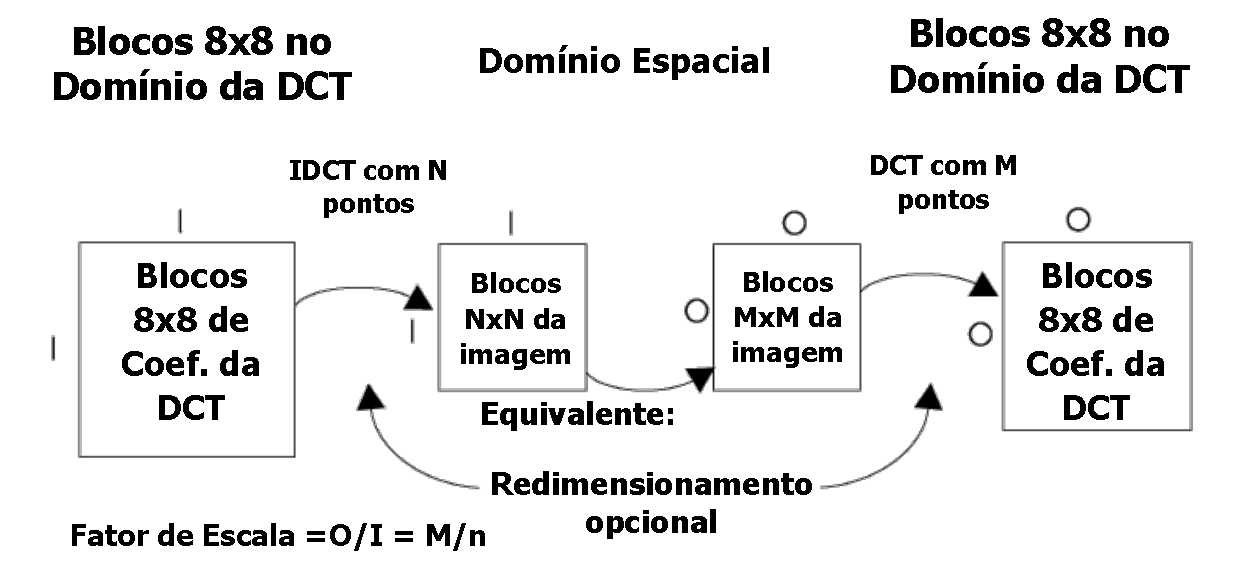
\includegraphics[scale=0.6]
{figuras/DCT_RES.pdf}
	\caption{Escala arbitrária redimensionando com uma ou ambas as transformadas locais. Nota-se que a dimensão é dada em blocos (por exemplo, o tamanho da primeira imagem é de $I$ blocos por $I$ blocos, onde cada cada bloco é de tamanho 8x8, o tamanho da segunda imagem ainda é $I$ blocos por $I$ blocos, mas o tamanho de cada bloco é $NxN$, etc \cite{salazar2007complexity}.}
	\label{DCT_RES}
\end{figure}

\section{Compressão e Codificação de Imagens e Vídeos Digitais}

O termo \enquote{compressão de dados} refere-se ao processo de redução do montante de dados exigidos para representar uma dada quantidade de informação. Deve-se esclarecer que denominamos \enquote{dados} aos meios pelos quais uma informação é transmitida \cite{richardson2011h}.

\subsection{Compressão Sem Perdas}
Técnicas de compressão sem perdas, como o seu nome indica, não envolvem perda de informações. Se os dados sofreram compressão do tipo sem perdas, pode-se recuperar exatamente os dados originais a partir  os dados comprimidos \cite{ukrit2011survey}.

Compressão de texto é uma área importante para a compressão sem perdas. É muito importante que a reconstrução seja idêntica a do texto original, pois diferenças muito pequenas podem resultar em orações com significados muito diferentes. Considere as frases \enquote{Não, enviem dinheiro} e \enquote{Não enviem dinheiro}. Um argumento semelhante vale para arquivos de computador e para certos tipos de dados, tais como registros bancários \cite{sayood2012introduction}.

Se os dados comprimidos vão ser processados (para se obter mais informação) ou \enquote{melhorados} é importante que a integridade seja preservada. Por exemplo, suponhamos que uma imagem radiológica seja comprimida de uma forma com perdas, e a diferença entre a imagem reconstruída e o original seja visualmente indetectável. Se esta imagem foi mais tarde reforçada, as diferenças anteriormente indetectáveis podem causar o aparecimento de artefatos que poderiam enganar seriamente o radiologista \cite{sayood2012introduction}.

\subsubsection{Entropia}

Segundo \cite{shannon2001mathematical}, considerando uma fonte discreta de informação, para cada estado possível $i$ haverá um conjunto de probabilidades ($P_i(j)$) de produzir os $j$ possíveis símbolos . Assim, há uma entropia ($H(j)$) para cada estado. A entropia da fonte será definida como a média desses $H$s, ponderados de acordo com a probabilidade de ocorrência dos estados em questão, como mostrado a seguir:

\begin{equation}
\label{ENTROPIA}
	\begin{split}
		H = \sum_i P_iH_i\\
		= - \sum_{i,j} P_i(j) log(P_i(j))
	\end{split}
\end{equation}

De acordo com mesmo autor, se a base do algoritmo na equação \ref{ENTROPIA} for 2, a entropia representará uma medida de \textit{bits} por símbolos, sendo essa a medida do número médio de \textit{bits} necessários para codificar a saída da fonte. 

A quantidade de informação nova transmitida por um símbolo diminui na medida em que a probabilidade de ocorrência deste símbolo aumenta. Então, os codificadores que exploram a redundância entrópica tem por objetivo transmitir o máximo de informação possível por símbolo codificado e, deste modo, representar
mais informações com um número menor de \textit{bits}. A codificação de entropia, como é chamada, utiliza diferentes técnicas e algoritmos de compressão sem perdas para atingir este objetivo \cite{da2007estudo}.

\subsection{Compressão com perdas}

Técnicas de compressão com perdas envolvem alguma perda de informações, assim, dados que tenham sido comprimidos utilizando técnicas com perdas geralmente não podem ser recuperados ou reconstruídos exatamente. Em troca de aceitar essa distorção na reconstrução, podemos geralmente obter taxas de compressão muito mais elevadas do que com compressão sem perdas  \cite{sayood2012introduction}.

De acordo com o mesmo autor, em muitas aplicações nota-se que a diferença entre a informação reconstruída e a original pode ser aceitável. Por exemplo, na compressão de video, diferenças entre os sinais original e reconstruído podem ser toleradas, contanto que elas não resultem em artefatos inconvenientes. Assim, sequências de vídeo são geralmente comprimidas usando compressão com perdas.

\subsection{Padrão JPEG} \label{JPEG}
 O padrão JPEG é um método de compressão com perdas, comumente empregado para imagens de tons contínuos, devido à sua alta eficácia e baixa complexidade computacional \cite{wang2008jpeg}.
 
Este padrão é definido pelo \cite{T.81}, sendo largamente utilizado em máquinas fotográficas, scanners e páginas da internet. 

De acordo \cite{wallace1991jpeg}, o algoritmo do padrão JPEG é descrito pelo fluxograma nas imagens \ref{ENCODER_JPEG} e \ref{DECODER_JPEG}.

\begin{figure}[h]
	\centering
	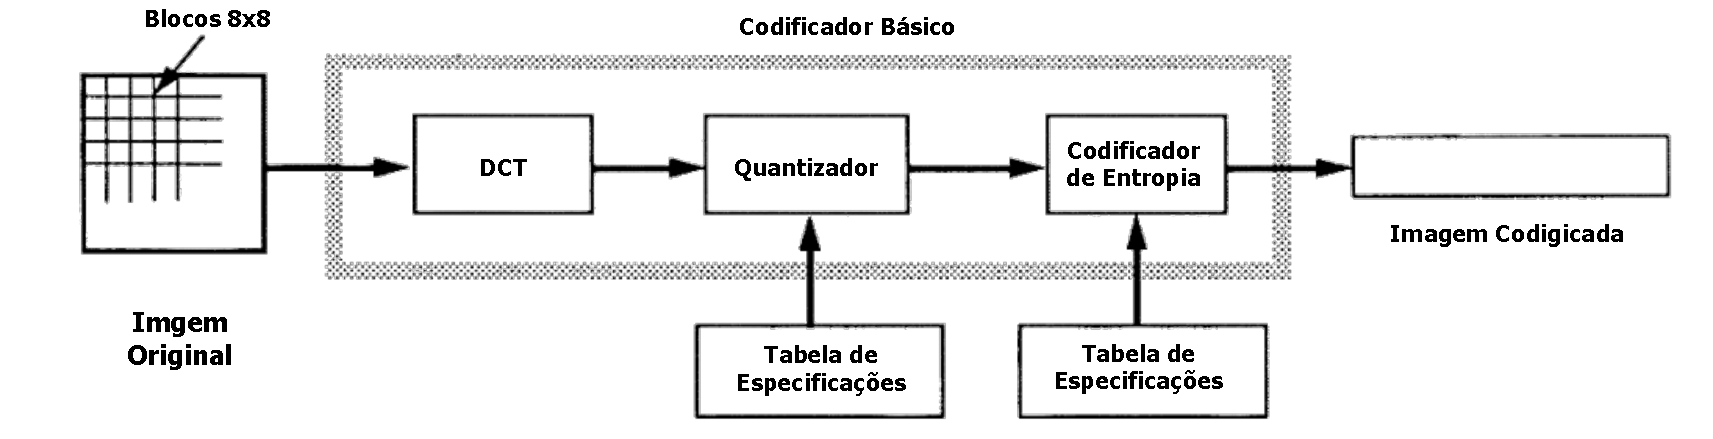
\includegraphics[scale=0.55]{figuras/ENCODER-JPEG.pdf}
	\caption{Etapas de codificação baseada em DCT \cite{wallace1991jpeg}.}
	\label{ENCODER_JPEG}
\end{figure}

\begin{figure}[h]
	\centering
	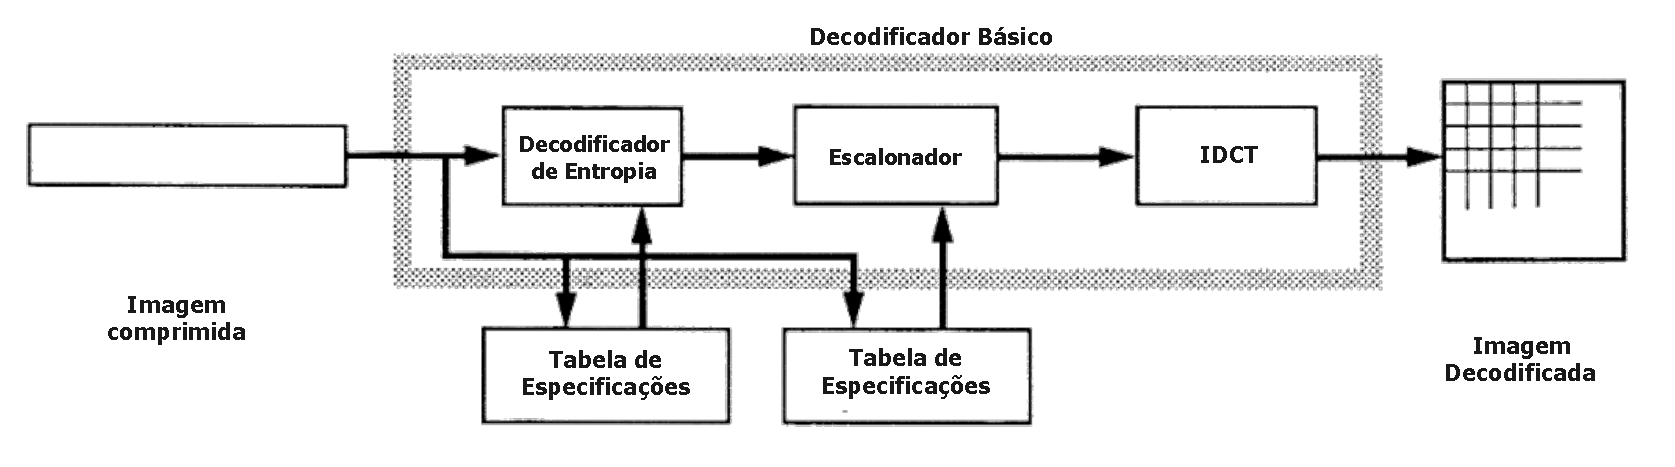
\includegraphics[scale=0.55]{figuras/DECODER-JPEG.pdf}
	\caption{Etapas de decodificação baseada em DCT \cite{wallace1991jpeg}.}
	\label{DECODER_JPEG}
\end{figure}
  
 A primeira etapa pela qual a imagem passa na codificação é a FDCT. Já na última etapa, na saída do decodificador, a IDCT, que de acordo com o mesmo autor, nada mais é que uma outra transformada matemática que faz o inverso da FDCT, converte coeficientes em amostras da imagem. 

De acordo \cite{wallace1991jpeg}, após a saída do FDCT, cada um dos 64 coeficientes (blocos 8x8) da DCT  é quantizado uniformemente em conjunto com uma matriz de normalização de 64 elementos, que deve ser indicada pela aplicação (ou usuário) como uma entrada para o codificador. Cada elemento pode variar entre 1 e 255, o que indica o tamanho de degrau do quantizador do seu coeficiente DCT respectivo. A finalidade de quantização (\textit{quantizer}) é conseguir uma compressão adicional, apenas por representar os coeficientes de DCT com uma precisão suficiente para atingir a desejada qualidade de imagem. Dito de outra forma, o objetivo desta etapa de processamento é descartar informações que não são visualmente significativas. 

A quantização de uma matriz é definida como a divisão de cada um de seus elementos por um respectivo coeficiente de quantização (definido pela matriz de normalização), seguido de arredondamento para o inteiro mais próximo:
\vspace{-3mm}
\begin{flushleft}
	\begin{equation}
		F^Q(u,v)=\left \lfloor \frac{F(u,v)}{Q(u,v)} +0,5 \right \rfloor
	\end{equation}
\end{flushleft}
onde:
			$F(u,v)$ é a matriz de coeficientes da DCT,
			$F^Q(u,v)$ é a matriz de coeficientes quantizados da DCT e
			$Q(u,v)$ é a matriz de normalização,
			e o operador $\left \lfloor . \right \rfloor$ executa o arredondamento para o menor valor inteiro mais próximo. Sendo assim, a operação $\left \lfloor  +0,5 \right \rfloor$ executa o arredondamento para o valor inteiro mais próximo.

			

Ainda de acordo com \cite{wallace1991jpeg}, a quantização inversa (\textit{dequantization}), presente na decoficação do JPEG, representa a função inversa da quantização, que nesse caso significa uma simples multiplicação (termo a termo) pela matriz de normalização, como mostrado a seguir.
\vspace{-5mm}
\begin{center}
	\begin{equation}
		\begin{split}
			F^{Q'}(u,v) =F^Q(u,v) * Q(u,v) \\
		\end{split}
	\end{equation}
\end{center} 
onde:
			$F^{Q'}(u,v)$ é a matriz de coeficientes desquantizados da DCT (aproximação de F(u,v)), 
			$F^Q(u,v)$ é a matriz de coeficientes quantizados da DCT e
			$Q(u,v)$ é a matriz de normalização.

Depois da quantização, o coeficiente DC é tratado separadamente dos 63 coeficientes AC. O coeficiente DC é uma medida do valor médio das 64 amostras de imagem. Como há correlação geralmente forte entre os coeficientes DC dos blocos 8x8 adjacentes, os coeficientes de DCT quantificados são codificados como a diferença de o termo DC do bloco anterior na ordem de codificação (zig-zag), como mostrado na Figura \ref{ZIG_ZAG} . Este tratamento especial vale a pena, pois coeficientes DC frequentemente contêm uma fração significativa do total de energia imagem \cite{wallace1991jpeg}.

\begin{figure}[h]
	\centering
	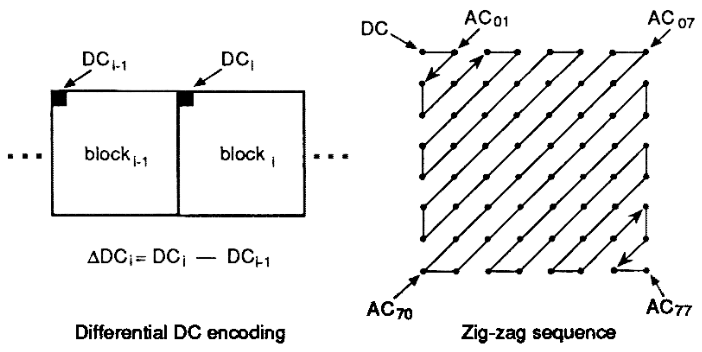
\includegraphics[scale=0.55]{figuras/ZIG-ZAG.png}
	\caption{Preparação dos coeficientes da DCT para o codificador de entropia \cite{wallace1991jpeg}.}
	\label{ZIG_ZAG}
\end{figure}

A etapa final de codificação é a codificação de entropia.  Esta etapa realiza a compressão sem perdas adicionais, codificando os coeficientes quantificados da DCT de forma mais compacta com base nas suas características estatísticas.

\subsection{Sistema H.264/AVC}

H.264/AVC é um padrão da indústria para codificação de vídeo, mas também é um formato popular para vídeo codificado, assim como um conjunto de ferramentas para a compressão de vídeo \cite{richardson2011h}. Esse padrão foi publicado pela ITU juntamento com a ISO e é conhecido por vários nomes, como: \textit{H.264}, \textit{MPEG-4 Part 10} e \textit{Advanced Video Coding (AVC)}. Desenvolvido por uma equipe composta de centenas de especialistas de compressão de vídeo, o \textit{Joint Video Team}, um esforço colaborativo entre a\textit{Moving Picture Experts Group (MPEG)} e o \textit{Video Coding Experts Group (VCEG)}.

A estrutura de um típico codec H.264 é mostradas nas figuras \ref{H264_ENCODER} e \ref{H264_DECODER} \cite{richardson2011h}.

\begin{figure}[h]
	\centering
	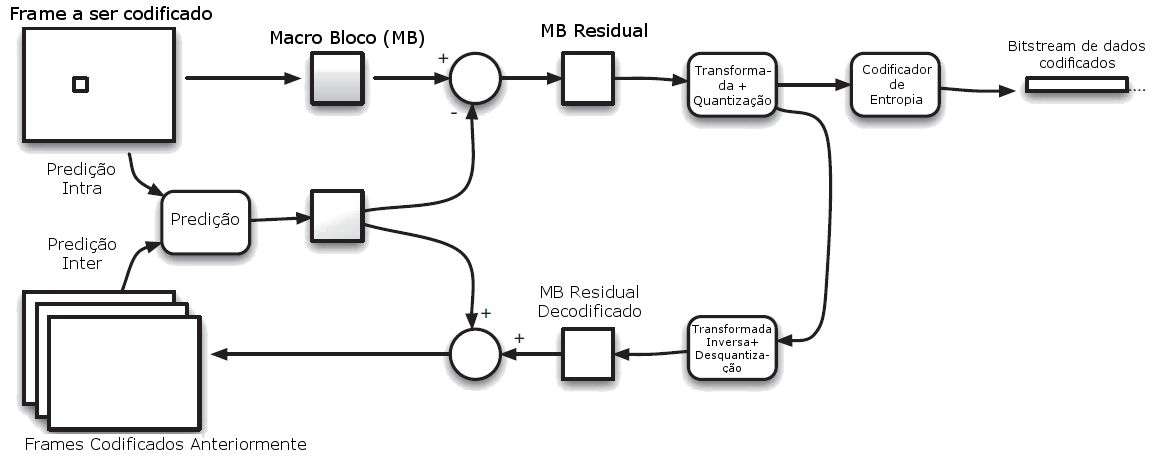
\includegraphics[scale=0.45]{figuras/H264_CODIFICADOR.png}
	\caption{Estrutura típica de um codificador H.264 \cite{richardson2011h}.}
	\label{H264_ENCODER}
\end{figure}

As imagens são processadas em unidades de macroblocos (MB), que correspondem a blocos de 16x16 \textit{pixels} \cite{richardson2011h}. No codificador, é gerada uma previsão para cada macrobloco a partir de blocos já codificados. Em seguida, a previsão é subtraída do macrobloco gerando o macrobloco residual, que é transformado, quantizado e codificado por codificação de entropia, em processos similares aos descritos na seção \ref{JPEG} .

Ainda, conforme o mesmo autor, sabe-se que a predição, ou previsão, do macrobloco atual gerada no codificador acontece a partir de dados previamente codificados, seja usando a informação da próprio quadro (\textit{frame}) atual (predição intra-quadro) ou utilizando informação de quadros anteriormente codificados (predição inter-quadros).
  
\begin{figure}[h]
	\centering
	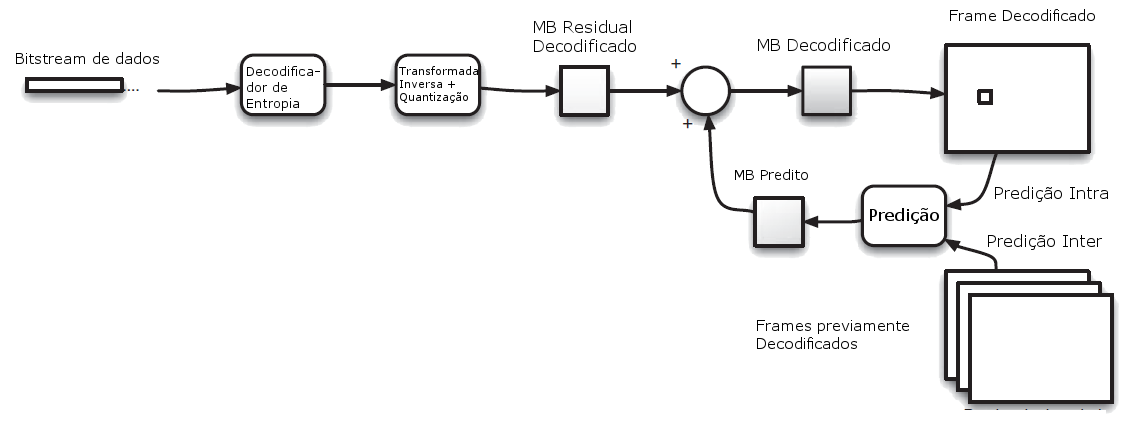
\includegraphics[scale=0.45]{figuras/H264_DECODIFICADOR.png}
	\caption{Estrutura típica de um decodificador H.264 \cite{richardson2011h}.}
	\label{H264_DECODER}
\end{figure}

No decodificador, um macrobloco é decodificado (operação inversa à codificação de entropia), desquantizado e passa pela transformada inversa de modo a formar um macrobloco residual descodificado (similar ao macrobloco residual gerado no codificador). Ainda no decodificador é gerada a mesma previsão que foi criada no codificador que é somada ao macrobloco residual decodificado para então produzir uma aproximação do macrobloco original da imagem \cite{richardson2011h}.

\section{Métricas de Qualidade}
Uma vez que tenhamos desenvolvido um esquema de compressão de dados, precisamos ser capazes de medir o seu desempenho. Devido ao grande número de diferentes áreas de aplicação, condições diferentes têm sido desenvolvidas para descrever e medir o desempenho \cite{sayood2012introduction}.

Um método comum utilizado como medida de desempenho para diversas técnicas de compressão de imagens é a relação sinal de pico/ruído (PSNR, do inglês \textit{Peak Signal Noise Ratio}), que é a relação entre o máximo possível de potência de um sinal pela potência do ruído, quando comparamos um sinal antes e depois de um
processo de degradação, ou seja, a imagem original e a imagem comprimida. Um valor alto de PSNR significa uma alta relação entre a potência da imagem original pela potência da imagem comprimida, ou seja, uma melhor qualidade da imagem reconstruída. Em termos matemáticos, o valor do PSNR entre uma imagem original  e uma imagem reconstruída é dado pela Eq. \ref{PSNR} \cite{vergutz2013combinaccao} : 
\vspace{-3mm}
\begin{center}
	\begin{equation}
		\label{PSNR}
		PSNR = 10\cdot log\left(\displaystyle\frac{255^2}{MSE}\right)
	\end{equation}
\end{center}

\noindent onde $MSE$ é uma medida referente a diferença entre a sequência original de vídeo e a processada, dada por:
\vspace{-5mm}
\begin{center}
	\begin{equation}
		MSE = \displaystyle\frac{1}{M\cdot N}\sum_{i=0}^{M-1}\sum_{j=0}^{N-1} (Y_{out}(i,j) - Y_{in}(i,j))^2 
	\end{equation}
\end{center} 	
onde $Y_{out}$ representa a imagem reconstruida, $Y_{in}$ representa a imagem, $N$ representa o número total de linhas de \textit{pixels} da imagem, $M$ o número de colunas  e $Y(i,j,m)$ é o valor  da luminância (0-255) na posição $(i,j)$ da imagem.

Já para avaliar a degradação em uma sequência de vídeo toma-se a PSNR médio das imagens que compõe a sequência, dado por:
\vspace{-5mm}
\begin{center}
	\begin{equation}
		PSNR_{Médio}(k) = \displaystyle\frac{1}{K}\sum_{K=0}^{K-1} 10log_{10}\left(\frac{255^2}{MSE(K)}\right)
	\end{equation}
\end{center}

\noindent onde $K$ é o número de quadros da sequência e o $MSE(K)$ é o $MSE$ do K-ésimo quando da sequência de vídeo.
